\chapter{Usage \ooad[121]}
\begin{figure}[H]
    \begin{tabular}{|l|p{12cm}|}
        \hline
        \textbf{Purpose} & \begin{itemize}
            \item To determine how actors interact with a system.
        \end{itemize} \\\hline
        \textbf{Concepts} & \begin{itemize}
            \item Actor: An abstraction of users or other systems that interact with the target system.
            \item Use case: A pattern for interaction between the system and actors in the application domain.
        \end{itemize} \\\hline
        \textbf{Principles} & \begin{itemize}
            \item Determine the application domain with use cases.
            \item Evaluate use cases in collaboration with users.
            \item Assess social changes in the application domain.
        \end{itemize} \\\hline
        \textbf{Result} & \begin{itemize}
            \item Descriptions of all use cases and actors, also known as actor tables.
        \end{itemize} \\\hline
    \end{tabular}
\end{figure}

\section{Use cases}
Focus on interaction between users and the system.
\begin{figure}[H]
    \textit{\textbf{Actor -} An abstraction of users or other systems that interact with the target system.}
\end{figure}
Actors are an abstraction of people and other systems that activates a target system function.\\
The complete set of use cases determines all uses of the target system within the application domain.
\begin{figure}[H]
    \textit{\textbf{Use case -} A pattern for interaction between the system and actors in the application domain.}
\end{figure}

\principle[Determine the application domain with use cases.]

\begin{figure}[H]
    \centering
    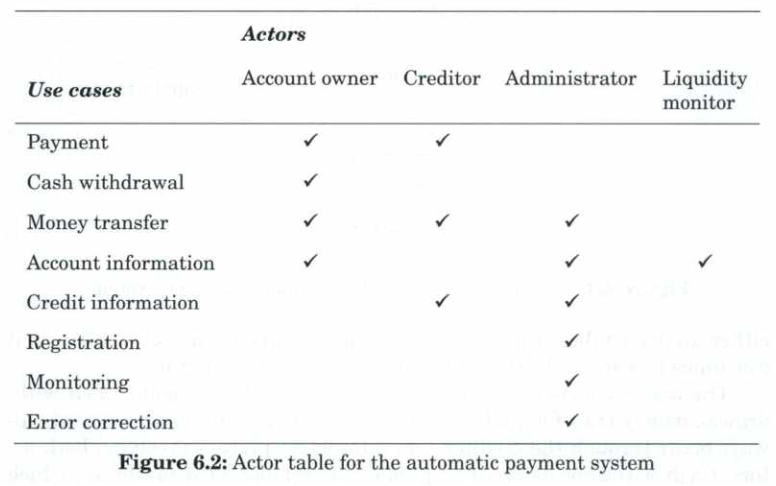
\includegraphics[width=\linewidth*3/4]{parts/3_application_domain_analysis/1_usage/figures/use_cases.png}
\end{figure}

\begin{figure}[H]
    \centering
    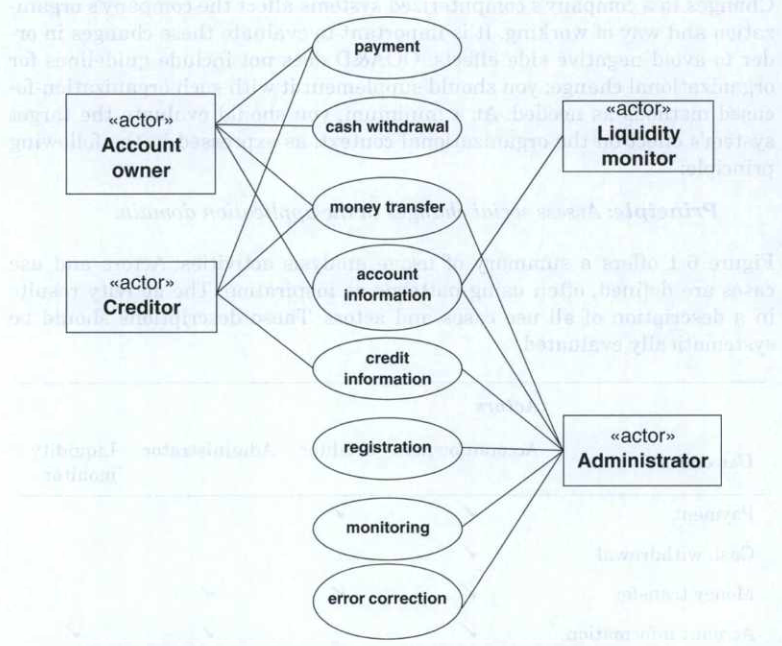
\includegraphics[width=\linewidth*3/4]{parts/3_application_domain_analysis/1_usage/figures/use_cases_diagram.png}
\end{figure}

\section{Find Actors and Use Cases}
Criterion for determening different actors is a dissimilarity of roles. If multiple roles appear the same to the system, they should be consolidated.
\subsection*{Describe actors}
\begin{figure}[H]
    \begin{tabular}{p{\textwidth }}
        \\\hline
        \begin{center}
            Account owner
        \end{center}
        \\\hline
        \begin{description}
            \item[Goal:] person who owns an account. The account owner’s basic need is to make payments with their plastic card.
            \item[Characteristics:] The system’s users include many account owners, with different levels of experience and sophistication.
            \item[Examples:] Account Owner A feels insecure about using a plastic card as a form of payment. Owner A originally got a card be cause it was the only way he could get an ID card for his checks. Owner A only withdraws money from the ATM in emergency situations.
            \item[] Account Owner B is technologically curious and she uses the system often, optimally, and to the limit of its abilities. B has never had major problems in understanding the system’s possibilities, and also examines possibilities that are not obviously accessible.
        \end{description}
        \\\hline
    \end{tabular}
\end{figure}
\subsection*{Describe Use Cases}
Can be described with statechart diagram for a good overview or a use-case specification for more details. It should make use of abstraction, the goal is to collect many possible ways of using the traget system in a few well-chosen use cases.

\subsection*{How to Select Work Tasks}
A work task uses a use a case, and in turn is used by the actor.\\
\\
\textbf{Help to select}\\
What tasks exist in the application domain?\\
What is the division of labor?\\
How are the different tasks delimited?\\
Describe the work tasks:
\begin{itemize}
    \item Name and content
    \item Purpose
    \item How is it assigned?
    \item Who perfomed it?
    \item Relationship and other tasks
    \item Result
\end{itemize}